\HeadingLevelB{Cryptographic Primitives}
\label{sec:crypto_primitives}

This section overviews the cryptosystems used by secure architectures. We are
interested in cryptographic primitives that guarantee privacy, integrity, and
freshness, and we treat these primitives as black boxes, focusing on their use
in larger systems. \cite{katz2014crypto} covers the mathematics behind
cryptography, while \cite{ferguson2011crypto} covers the topic of building
systems out of cryptographic primitives. Tables \ref{fig:crypto_names}
and \ref{fig:crypto_primitives} summarize the primitives covered in this
section.

\begin{table}[hbt]
  \centering
  \begin{tabular}{| l | l |}
  \hline
  \textbf{Guarantee} & \textbf{Primitive} \\
  \hline
  Privacy & \textit{Encryption} \\
  \hline
  Integrity & \textit{MAC} / \textit{Signatures} \\
  \hline
  Freshness & \textit{Nonces} + integrity \\
  \hline
  \end{tabular}
  \caption{
    Desirable security guarantees and primitives that provide them
  }
  \label{fig:crypto_names}
\end{table}

\begin{table}[hbt]
  \centering
  \begin{tabular}{| l | l | l |}
  \hline
  \textbf{Guarantee} & \textbf{Symmetric} & \textbf{Asymmetric} \\
                     & \textbf{Keys} & \textbf{Keys} \\
  \hline
  Privacy & AES-GCM, & RSA with \\
          & AES-CTR  & PKCS \#1 v2.0 \\
  \hline
  Integrity & HMAC-SHA-2 & DSS-RSA, \\
            & AES-GCM & DSS-ECC \\
  \hline
  \end{tabular}
  \caption{
    Popular cryptographic primitives that are considered to be secure against
    today's adversaries
  }
  \label{fig:crypto_primitives}
\end{table}

A message whose \textit{privacy} is protected can be transmitted over an
insecure medium without an adversary being able to obtain the information in
the message. When \textit{integrity} protection is used, the receiver is
guaranteed to either obtain a message that was transmitted by the sender, or to
notice that an attacker tampered with the message's content.

When multiple messages get transmitted over an untrusted medium, a
\textit{freshness} guarantee assures the receiver that she will obtain the
latest message coming from the sender, or will notice an attack. A freshness
guarantee is stronger than the equivalent integrity guarantee, because the
latter does not protect against \textit{replay attacks} where the attacker
replaces a newer message with an older message coming from the same sender.

The following example further illustrates these concepts. Suppose Alice is a
wealthy investor who wishes to either \textsc{buy} or \textsc{sell} an item
every day. Alice cannot trade directly, and must relay her orders to her
broker, Bob, over a network connection owned by Eve.

A communication system with privacy guarantees would prevent Eve from
distinguishing between a \textsc{buy} and a \textsc{sell} order, as illustrated
in Figure~\ref{fig:privacy_attack}. Without privacy, Eve would know Alice's
order before it is placed by Bob, so Eve would presumably gain a financial
advantage at Alice's expense.

\begin{figure}[hbt]
  \centering
  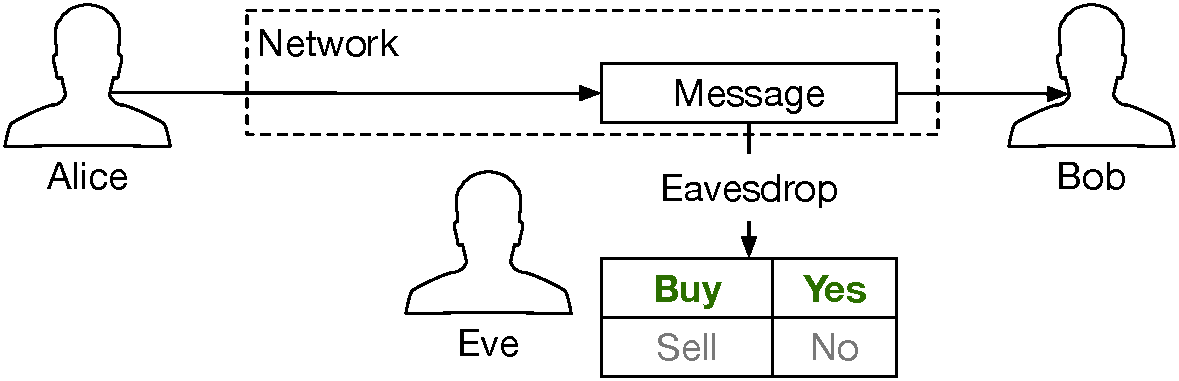
\includegraphics[width=85mm]{figures/privacy_attack.pdf}
  \caption{
    In a privacy attack, Eve sees the message sent by Alice to Bob and can
    understand the information inside it. In this case, Eve can tell that the
    message is a \textbf{buy} order, and not a \textbf{sell} order.
  }
  \label{fig:privacy_attack}
\end{figure}

A system with integrity guarantees would prevent Eve from replacing Alice's
message with a false order, as shown in Figure~\ref{fig:integrity_attack}. In
this example, without integrity guarantees, Eve could replace Alice's message
with a \textsc{sell-everything} order, and buy Alice's assets at a very low
price.

\begin{figure}[hbt]
  \centering
  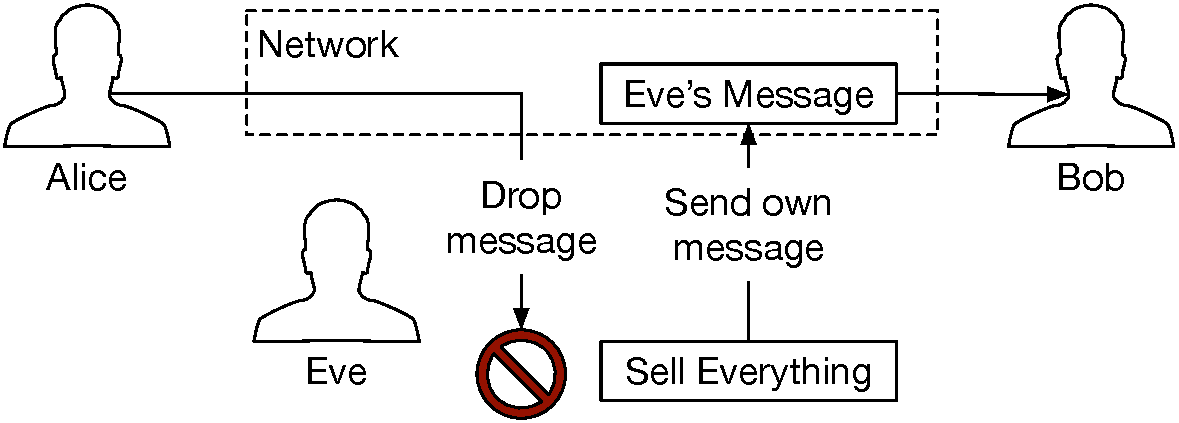
\includegraphics[width=85mm]{figures/integrity_attack.pdf}
  \caption{
    In an integrity attack, Eve replaces Alice's message with her own. In this
    case, Eve sends Bob a \textbf{sell-everything} order. In this case, Eve can
    tell that the message is a \textbf{buy} order, and not a \textbf{sell}
    order.
  }
  \label{fig:integrity_attack}
\end{figure}

Last, a communication system that guarantees freshness would ensure that Eve
cannot perform the replay attack pictured in Figure~\ref{fig:freshness_attack},
where she would replace Alice's message with an older message. Without
freshness guarantees, Eve could mount the following attack, which bypasses
both privacy and integrity guarantees. Over a few days, Eve would copy and
store Alice's messages from the network. When an order would reach Bob, Eve
would observe the market and determine if the order was \textsc{buy} or
\textsc{sell}. After building up a database of messages labeled \textsc{buy} or
\textsc{sell}, Eve would replace Alice's message with an old message of her
choice.

\begin{figure}[hbt]
  \centering
  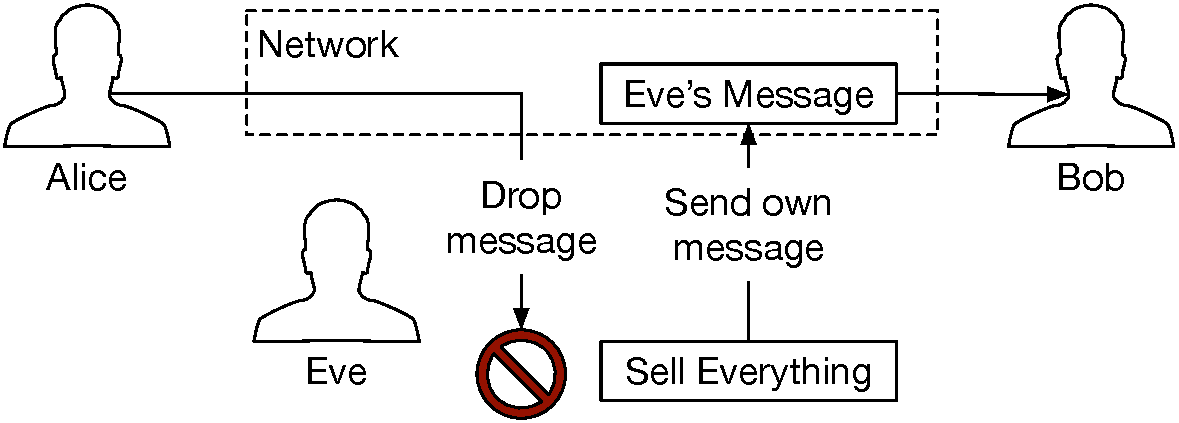
\includegraphics[width=85mm]{figures/integrity_attack.pdf}
  \caption{
    In a freshness attack, Eve replaces Alice's message with a message that she
    sent at an earlier time. In this example, Eve builds a database of labeled
    messages over time, and is able to send Bob her choice of a \textsc{buy} or
    a \textsc{sell} order.
  }
  \label{fig:freshness_attack}
\end{figure}


\HeadingLevelC{Cryptographic Keys}
\label{sec:crypto_keys}

All cryptographic primitives that we describe here rely on \textit{keys}, which
are small pieces of information that must only be disclosed according to
specific rules. A large part of a system's security analysis focuses on
ensuring that the keys used by the underlying cryptographic primitives are
produced and handled according to the primitives' assumptions.

Each cryptographic primitive has an associated \textit{key generation
algorithm} that uses random data to produce a unique key. The random data is
produced by a \textit{cryptographically strong pseudo-random number generator}
(CSPRNG) that expands a small amount of \textit{random seed} data into a much
larger amount of data, which is computationally indistinguishable from true
random data. The random seed must be obtained from a true source of randomness
whose output cannot be predicted by an adversary, such as the least significant
bits of the temperature readings coming from a hardware sensor.

\textit{Symmetric key} cryptography requires that all the parties in the system
establish a shared \textit{secret key}, which is usually referred to as ``the
key''. Typically, one party executes the key generation algorithm and securely
transmits the resulting key to the other parties, as illustrated in
Figure~\ref{fig:symmetric_key_generation}. The channel used to
distribute the key must provide privacy and integrity guarantees, which is a
non-trivial logistical burden. The symmetric key primitives mentioned here do
not make any assumption about the key, so the key generation algorithm simply
grabs a fixed number of bits from the CSPRNG.

\begin{figure}[hbt]
  \centering
  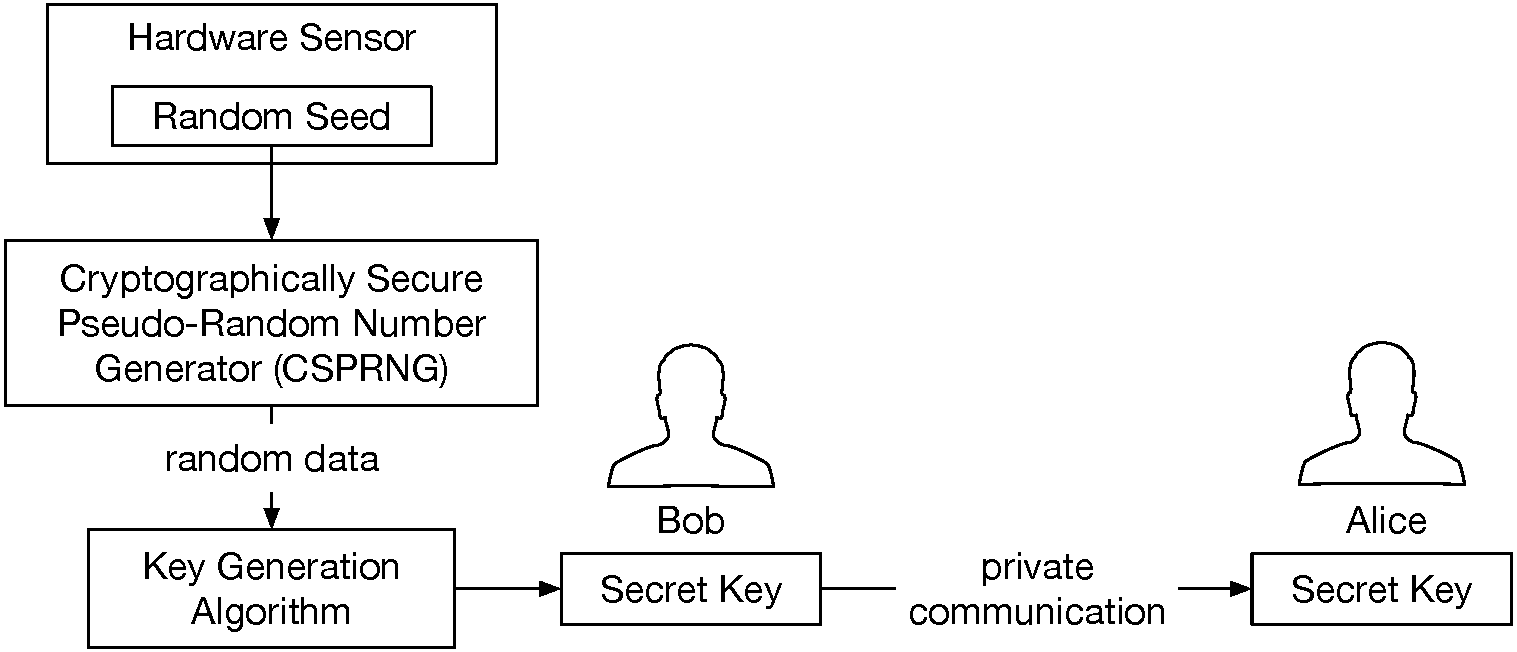
\includegraphics[width=87mm]{figures/symmetric_key_generation.pdf}
  \caption{
    In symmetric key cryptography, a secret key is shared by the parties that
    wish to communicate securely.
  }
  \label{fig:symmetric_key_generation}
\end{figure}

The defining feature of \textit{asymmetric key} cryptography is that it does not
require a private channel for key distribution. Each party executes the key
generation algorithm, which produces a \textit{private key} and a
\textit{public key} that are mathematically related. Each party's public key
is distributed to the other parties over a channel with integrity guarantees,
as shown in Figure~\ref{fig:asymmetric_key_generation}.
Asymmetric key primitives are more flexible than their symmetric counterparts,
but are more complicated and consume more computational resources.

\begin{figure}[hbt]
  \centering
  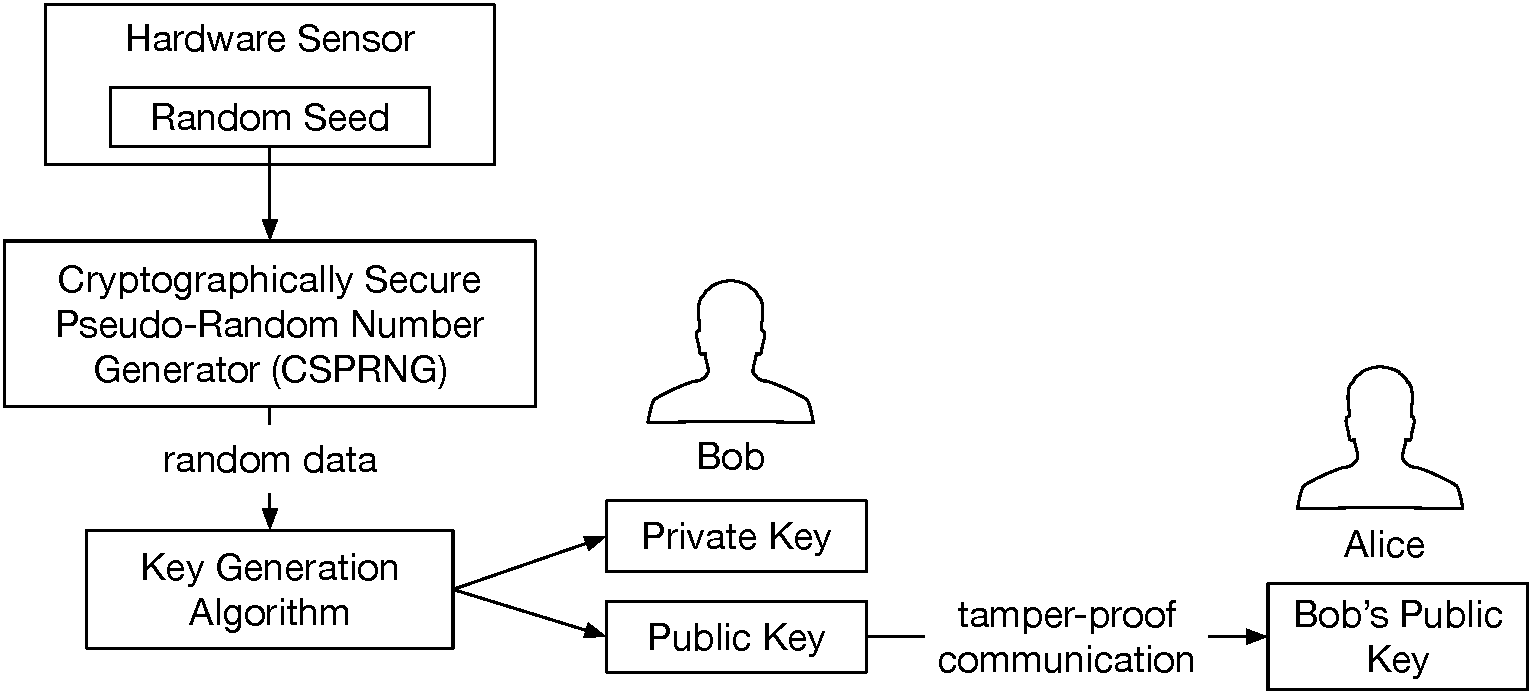
\includegraphics[width=87mm]{figures/asymmetric_key_generation.pdf}
  \caption{
    An asymmetric key generation algorithm produces a private key and an
    associated public key. The private key is held confidential, while the
    public key is given to any party who wishes to securely communicate with
    the private key's holder.
  }
  \label{fig:asymmetric_key_generation}
\end{figure}


\HeadingLevelC{Privacy}
\label{sec:privacy_crypto}

Many cryptosystems that provide integrity guarantees are built upon
\textit{block ciphers} that operate on fixed-size message blocks. The sender
transforms a block using an \textit{encryption} algorithm, and the receiver
inverts the transformation using a \textit{decryption} algorithm. The
encryption algorithms in block ciphers obfuscate the message block's content in
the output, so that an adversary who does not have the decryption key cannot
obtain the original message block from the encrypted output.

Symmetric key encryption algorithms use the same secret key for encryption and
decryption, as shown in Figure~\ref{fig:symmetric_block_cipher}, while
asymmetric key block ciphers use the public key for encryption, and the
corresponding private key for decryption, as shown in
Figure~\ref{fig:asymmetric_block_cipher}.
\begin{figure}[hbt]
  \centering
  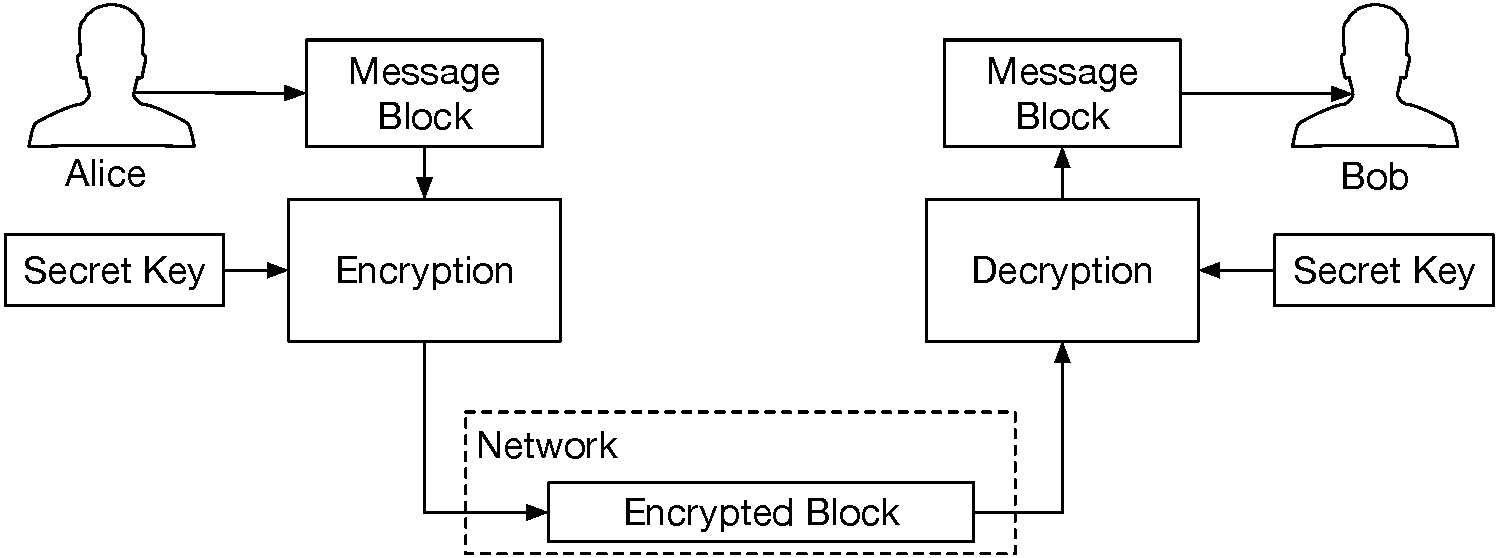
\includegraphics[width=85mm]{figures/symmetric_block_cipher.pdf}
  \caption{
    In a symmetric key secure permutation (block cipher), the same secret key
    must be provided to both the encryption and the decryption algorithm.
  }
  \label{fig:symmetric_block_cipher}
\end{figure}

\begin{figure}[hbt]
  \centering
  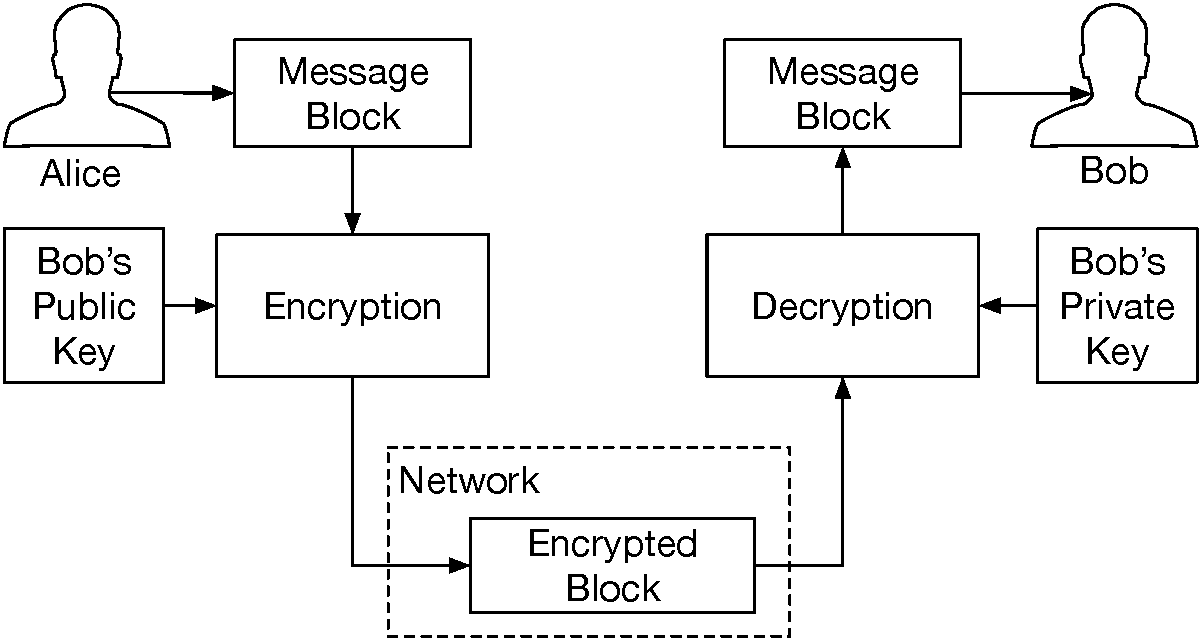
\includegraphics[width=85mm]{figures/asymmetric_block_cipher.pdf}
  \caption{
    In an asymmetric key block cipher, the encryption algorithm operates on a
    public key, and the decryption algorithm uses the corresponding private
    key.
  }
  \label{fig:asymmetric_block_cipher}
\end{figure}

The most popular block cipher based on symmetric keys at the time of this
writing is the
\textit{American Encryption Standard}~(AES)~\cite{daemen1999aes, fips2001aes},
with two variants that operate on 128-bit blocks using 128-bit keys or 256-bit
keys. AES is a \textit{secure permutation} function, as it can transform any
128-bit block into another 128-bit block. Recently, the United States
\textit{National Security Agency}~(NSA) required the use of 256-bit AES keys
for protecting sensitive information~\cite{nsa2015suiteb}.

The most deployed asymmetric key block cipher is the
\textit{Rivest-Shamir-Adelman}~(RSA)~\cite{rivest1978rsa} algorithm. RSA has
variable key sizes, and 3072-bit key pairs are considered to provide the same
security as 128-bit AES keys~\cite{fips2012keysize}.

A block cipher does not necessarily guarantee privacy, when used  on its own.
A noticeable issue is that in our previous example, a block cipher would
generate the same encrypted output for any of Alice's \textsc{buy} orders, as
they all have the same content. Furthermore, each block cipher has its own
assumptions that can lead to subtle vulnerabilities if the cipher is used
directly.

Symmetric key block ciphers are combined with operating modes to form symmetric
encryption schemes. Most operating modes require a random
\textit{initialization vector} (IV) to be used for each message, as shown in
Figure~\ref{fig:symmetric_encryption}. When analyzing the security of systems
based on these cryptosystems, an understanding of the IV generation process is
as important as ensuring the confidentiality of the encryption key.

\begin{figure}[hbt]
  \centering
  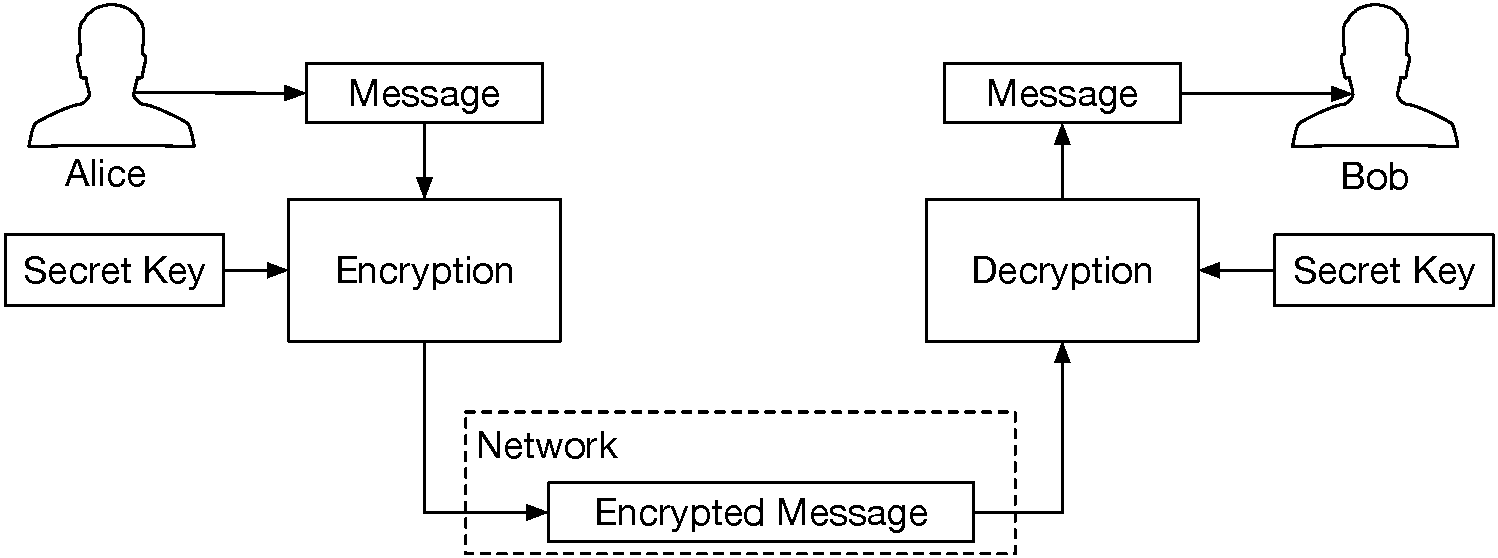
\includegraphics[width=85mm]{figures/symmetric_encryption.pdf}
  \caption{
    Symmetric key block ciphers are combined with operating modes. Most
    operating modes require a random initialization vector (IV) to be generated
    for each encrypted message.
  }
  \label{fig:symmetric_encryption}
\end{figure}

Counter (CTR) and Cipher Block Chaining (CBC) are examples of operating modes
recommended~\cite{fips2001ctr} by the United States \textit{National Institute
of Standards and Technology}~(NIST), which informs the NSA's requirements.
Combining a block cipher, such as AES, with an operating mode, such as CTR,
results in an encryption method, such as AES-CTR, which can be used to add
privacy guarantees.

In the asymmetric key setting, there is no concept equivalent to operating
modes. Each block cipher has its own assumptions, and requires a specialized
scheme for general-purpose usage.

The RSA algorithm is used in conjunction with \textit{padding methods}, the
most popular of which are the methods described in the \textit{Public-Key
Cryptography Standard} (PKCS) \#1 versions 1.5~\cite{kaliski1998pkcs1v15} and
2.0~\cite{kaliski1998pkcs1v2}. A security analysis of a system that uses
RSA-based encryption must take the padding method into consideration. For
example, the padding in PKCS \#1 v1.5 can leak the private key under certain
circumstances~\cite{bleichenbacher1998pkcs1v15cca}. While PKCS \#1 v2.0 solves
this issue, it is complex enough that some implementations have their own
security issues~\cite{manger2001pkcs1v20attack}.

Asymmetric encryption algorithms have much higher computational requirements
than symmetric encryption algorithms. Therefore, when non-trivial quantities of
data is encrypted, the sender generates a single-use secret key that is used
to encrypt the data, and encrypts the secret key with the receiver's public
key, as shown in Figure~\ref{fig:asymmetric_encryption}.

\begin{figure}[hbt]
  \centering
  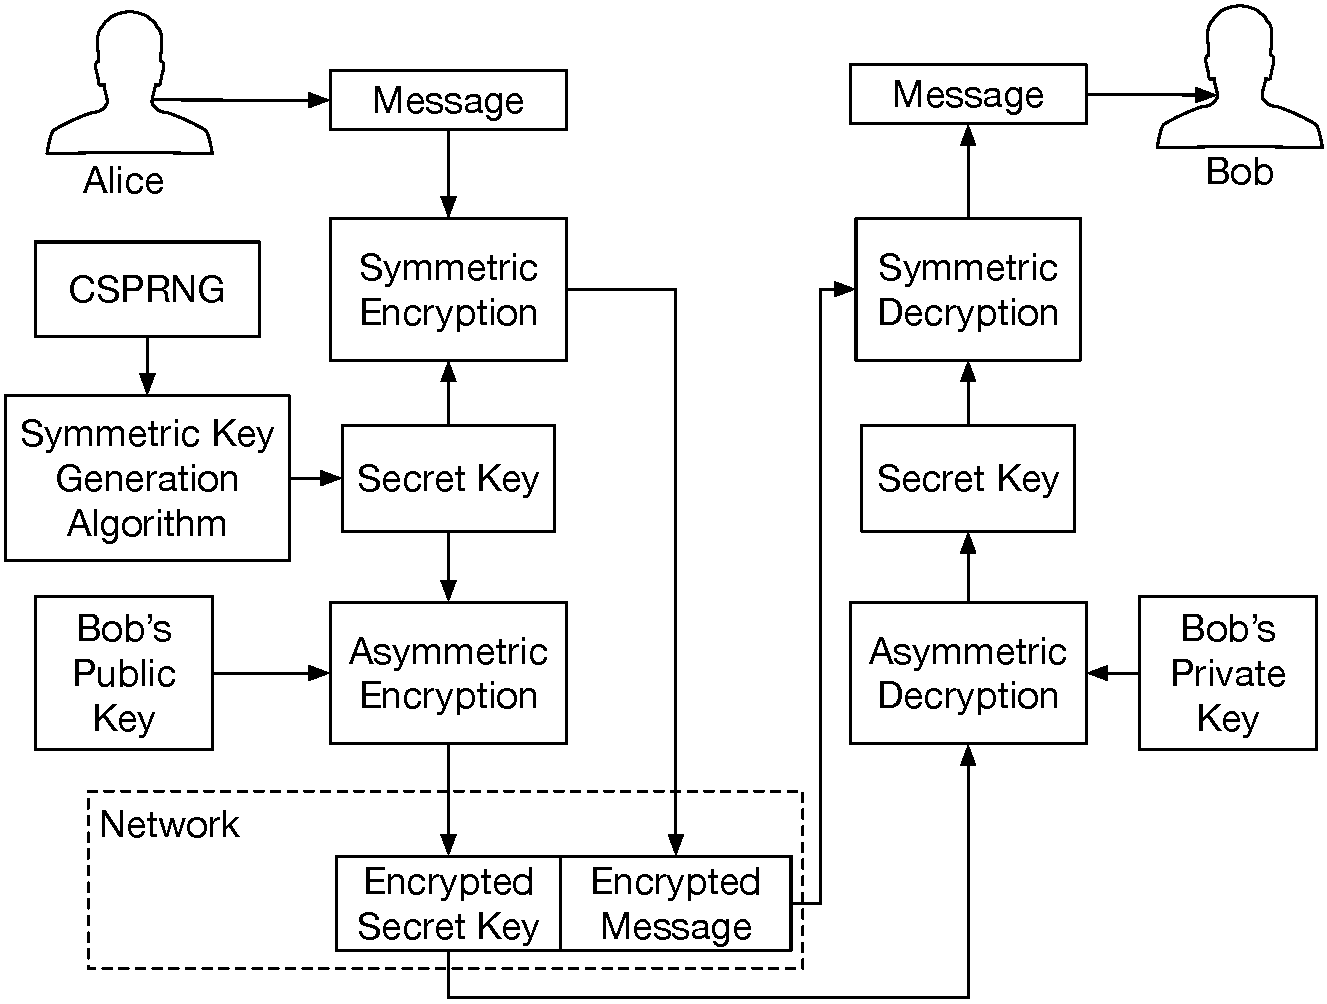
\includegraphics[width=87mm]{figures/asymmetric_encryption.pdf}
  \caption{
    Asymmetric key encryption is generally used to bootstrap a symmetric
    key encryption scheme.
  }
  \label{fig:asymmetric_encryption}
\end{figure}


\HeadingLevelC{Integrity}
\label{sec:integrity_crypto}

Many cryptosystems that provide integrity guarantees are built upon
\textit{secure hashing} functions. These hash functions operate on an unbounded
amount of input data and produce a small fixed-size output. Secure hash
functions have a few guarantees, such as \textit{pre-image resistance}, which
states that an adversary cannot produce input data corresponding to a given
hash output.

At the time of this writing, the most popular secure hashing function is the
\textit{Secure Hashing Algorithm}~(SHA)~\cite{eastlake2001sha1}. However, due
to security issues in SHA-1~\cite{stevens2015sha1attack}, new software is
recommended to use at least 256-bit SHA-2~\cite{fips2015shs} for secure
hashing.

The SHA hash functions are members of a large family of \textit{block hash
functions} that consume their input in fixed-size message blocks, and use a
fixed-size internal state. A block hash function is used as shown in
Figure~\ref{fig:block_hash_operation}. An \textsc{initialize} algorithm is
first invoked to set the internal state to its initial values. An
\textsc{extend} algorithm is executed for each message block in the input.
After the entire input is consumed, a \textsc{finalize} algorithm produces the
hash output from the internal state.

\begin{figure}[hbt]
  \centering
  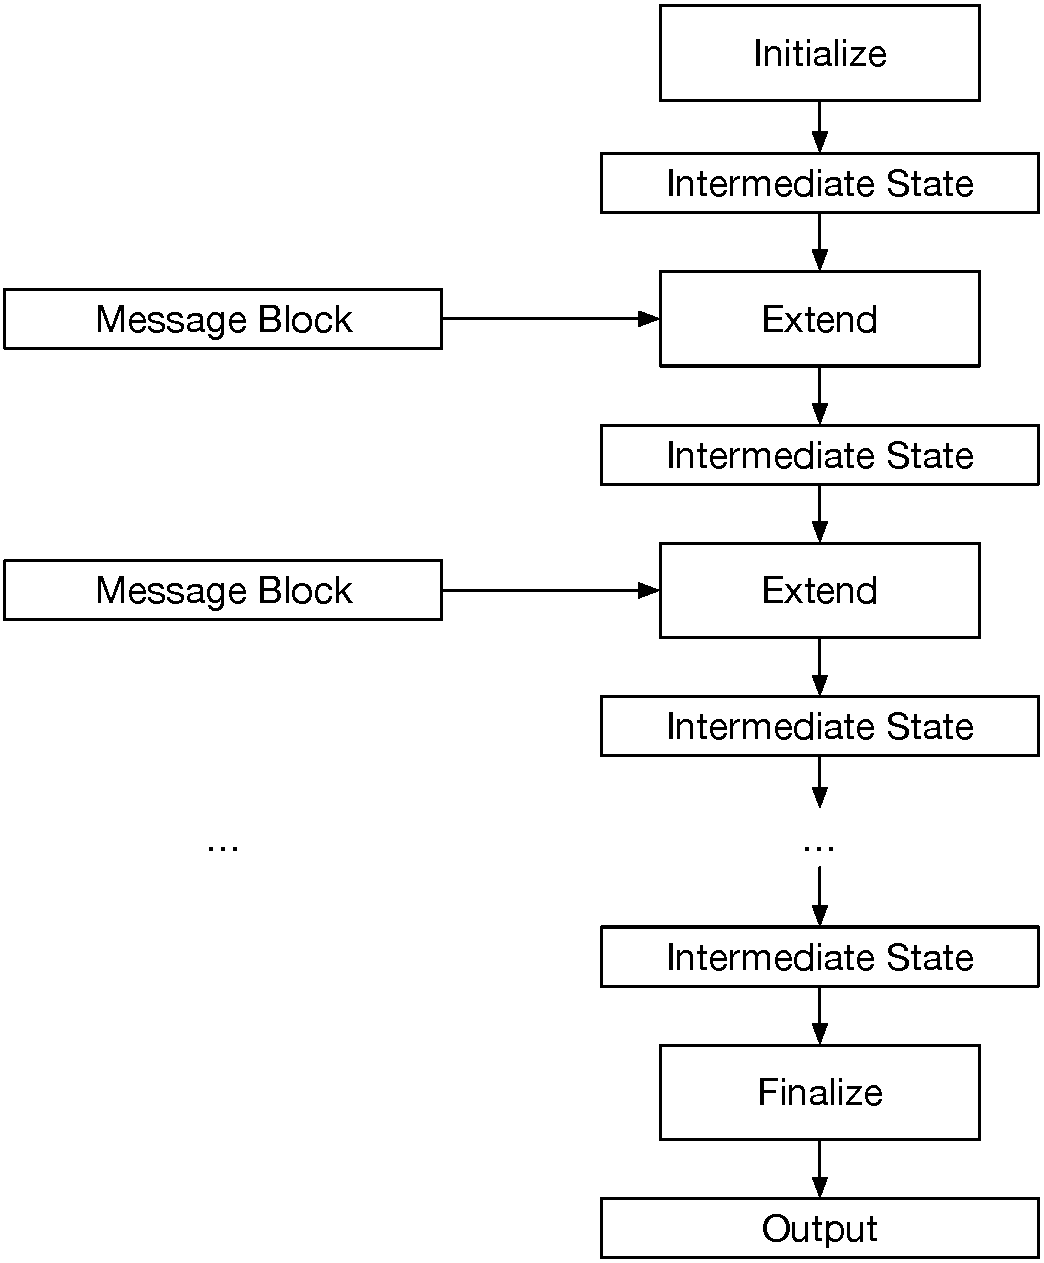
\includegraphics[width=70mm]{figures/block_hash_operation.pdf}
  \caption{
    A block hash function operates on fixed-size message blocks and uses a
    fixed-size internal state.
  }
  \label{fig:block_hash_operation}
\end{figure}

In the symmetric key setting, integrity guarantees are obtained using a
\textit{Message Authentication Code}~(MAC) cryptosystem, illustrated in
Figure~\ref{fig:symmetric_mac}. The sender uses a MAC algorithm that reads in a
symmetric key and a variable-legnth message, and produces a fixed-length, short
\textit{MAC tag}. The receiver provides the original message, the symmetric
key, and the MAC tag to a MAC verification algorithm that checks the
authenticity of the message.

\begin{figure}[hbt]
  \centering
  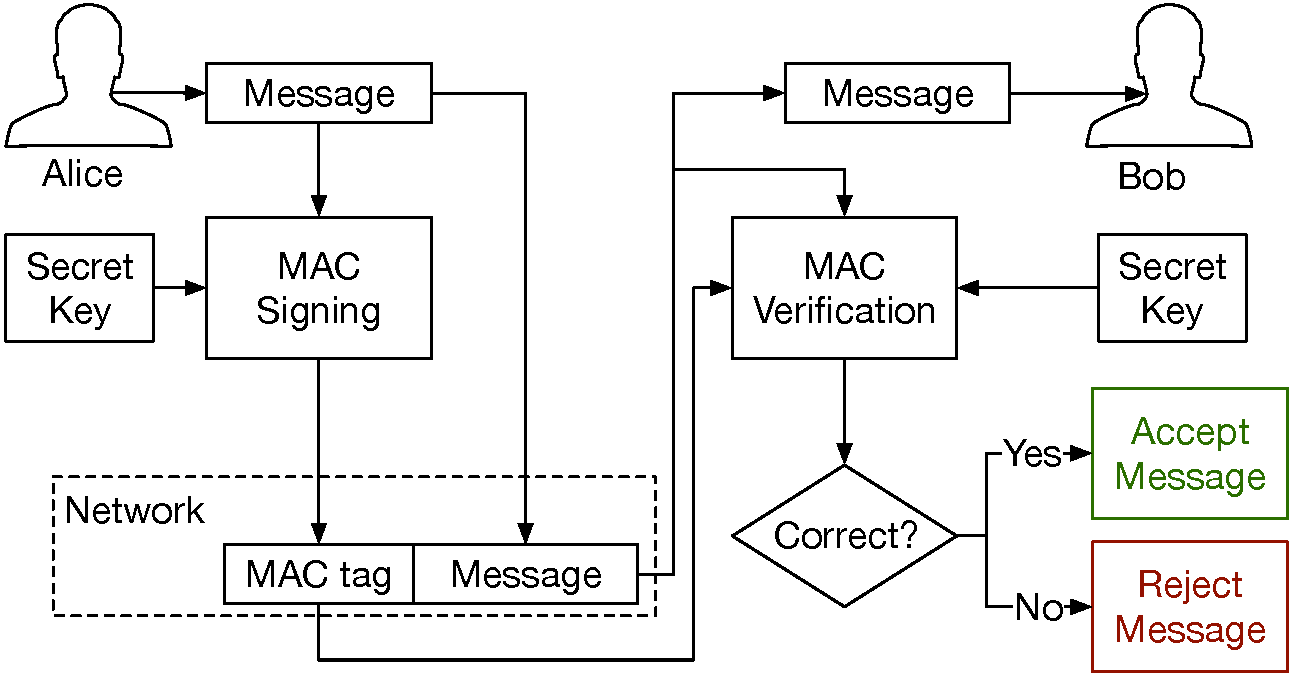
\includegraphics[width=87mm]{figures/symmetric_mac.pdf}
  \caption{
    In the symmetric key setting, integrity is assured by computing a
    Message Authentication Code (MAC) tag and transmitting it over the network
    along the message. The receiver feeds the MAC tag into a verification
    algorithm that checks the message's authenticity.
  }
  \label{fig:symmetric_mac}
\end{figure}

The key property of MAC cryptosystems is that an adversary cannot produce a
MAC tag that will validate a message without the secret key.

Many MAC cryptosystems do not have a separate MAC verification algorithm.
Instead, the receiver checks the authenticity of the MAC tag by running the
same algorithm as the sender to compute the expected MAC tag for the received
message, and compares the output with the MAC tag received from the network.

This is the case for the
\textit{Hash Message Authentication Code}~(HMAC)~\cite{krawczyk1997hmac}
generic construction, whose operation is illustrated in
Figure~\ref{fig:symmetric_hmac}. HMAC can use any secure hash function, such as
SHA, to build a MAC cryptosystem.

\begin{figure}[hbt]
  \centering
  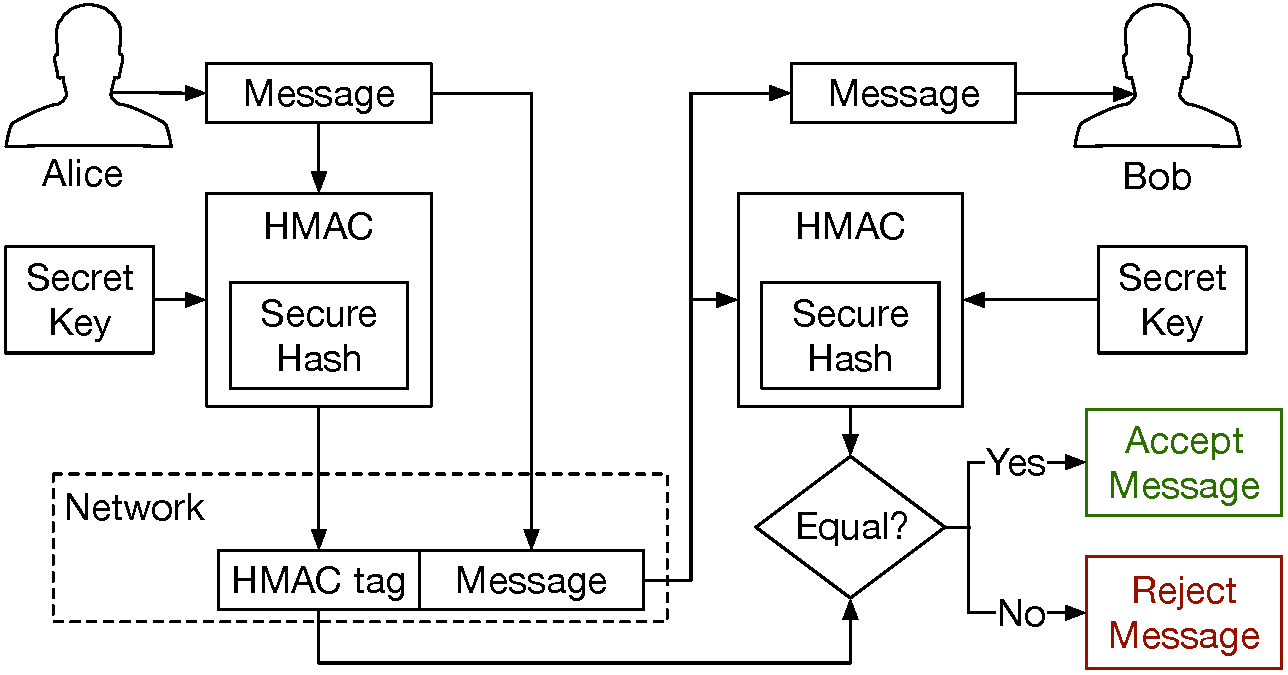
\includegraphics[width=87mm]{figures/symmetric_hmac.pdf}
  \caption{
    In the symmetric key setting, integrity is assured by computing a
    Hash-bassed Message Authentication Code (HMAC) and transmitting it over the
    network along the message. The receiver re-computes the HMAC and compares
    it against the version received from the network.
  }
  \label{fig:symmetric_hmac}
\end{figure}

Asymmetric key primitives that provide integrity guarantees are known as
\textit{signatures}. The message sender provides her private key to a
\textit{signing} algorithm, and transmits the output signature along with the
message, as shown in Figure~\ref{fig:asymmetric_signing}. The message receiver
feeds the sender's public key and the signature to a \textit{signature
verification} algorithm, which returns \textsc{true} if the message matches the
signature, and \textsc{false} if the message has been tampered with.

\begin{figure}[hbt]
  \centering
  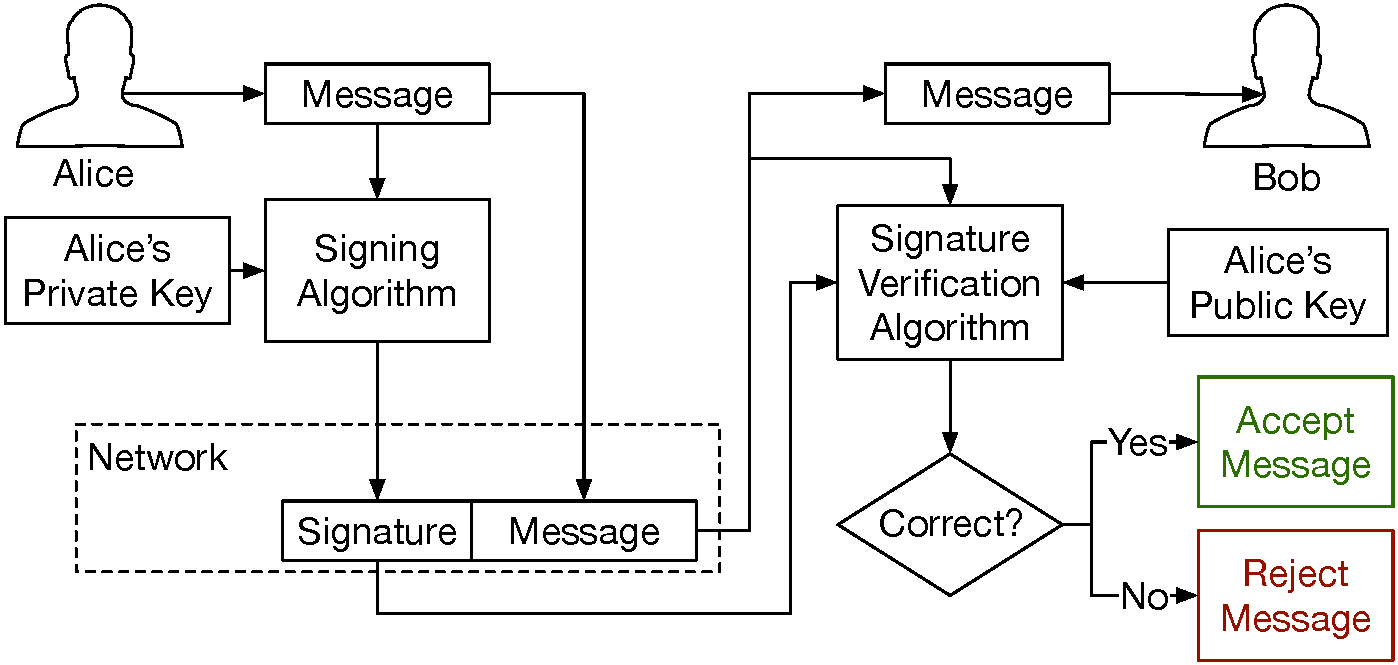
\includegraphics[width=87mm]{figures/asymmetric_signing.pdf}
  \caption{
    Signature schemes guarantee integrity in the asymmetric key setting.
    Signatures are created using the sender's private key, and are verified
    using the corresponding public key. A cryptographically secure hash
    function is usually employed to reduce large messages to small hashes,
    which are then signed.
  }
  \label{fig:asymmetric_signing}
\end{figure}

Signing algorithms can only operate on small messages and are computationally
expensive. Therefore, in practice, the message to be transmitted is first ran
through a cryptographically strong hash function, and the hash is provided as
the input to the signing algorithm.

At the time of this writing, the most popular choice for guaranteeing integrity
in shared secret settings is HMAC-SHA, an HMAC function that uses SHA for
hashing.

\textit{Authenticated encryption}, which combines a block cipher with an
operating mode that offers both privacy and integrity guarantees, is often an
attractive alternative to HMAC. The most popular authenticated encryption
operating mode is \textit{Galois/Counter operation
mode}~(GCM)~\cite{mcgrew2004gcm}, which has earned NIST's
recommendation~\cite{fips2017gcm} when combined with AES to form AES-GCM.

The most popular signature scheme combines the RSA encryption algorithms with a
padding schemes specified in PKCS \#1, as illustrated in
Figure~\ref{fig:rsa_pkcs1_v15_padding}. Recently, elliptic curve cryptography
(ECC)~\cite{koblitz1987ecc} has gained a surge in popularity, thanks to its
smaller key sizes. For example, a 384-bit ECC key is considered to be as secure
as a 3072-bit RSA key~\cite{fips2012keysize, nsa2015suiteb}. The NSA requires
the Digital Signature Standard~(DSS)\cite{fips2013dss}, which specifies schemes
based on RSA and ECC.

\begin{figure}[hbt]
  \centering
  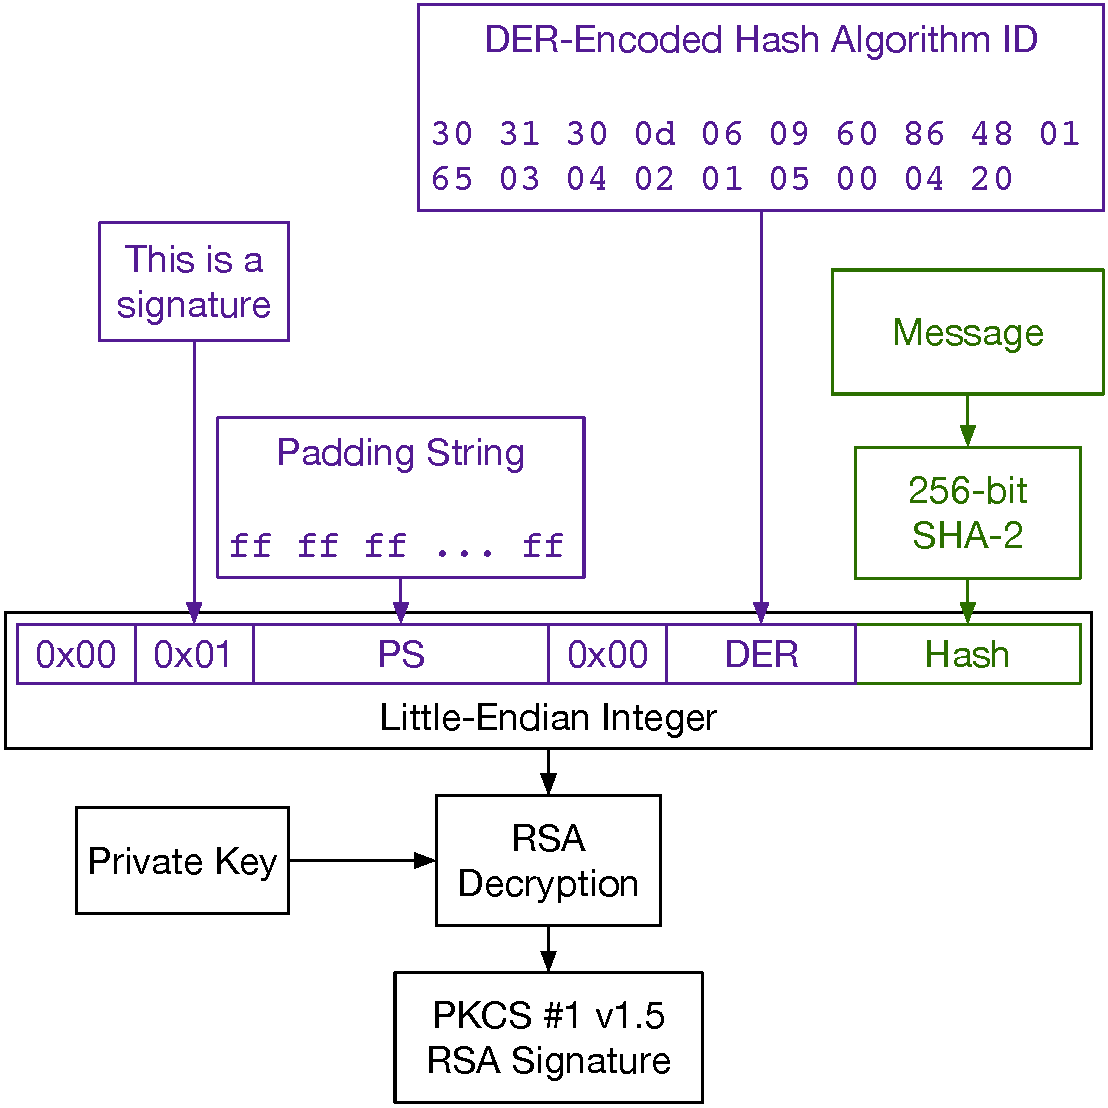
\includegraphics[width=85mm]{figures/rsa_pkcs1_v15_padding.pdf}
  \caption{
    The RSA signature scheme with PKCS \#1 v1.5 padding specified in RFC 3447
    combines a secure hash of the signed message with a DER-encoded
    specification of the secure hash algorithm used by the signature, and a
    padding string whose bits are all set to 1. Everything except for the
    secure hash output is considered to be a part of the PKCS \#1 v1.5 padding.
  }
  \label{fig:rsa_pkcs1_v15_padding}
\end{figure}


\HeadingLevelC{Freshness}
\label{sec:freshness_crypto}

Freshness guarantees are typically built on top of a system that already offers
integrity guarantees, by adding a unique piece of information to each message.
The main challenge in freshness schemes comes down to economically maintaining
the state needed to generate the unique pieces of information on the sender
side, and verify their uniqueness on the receiver side.

A popular solution for gaining freshness guarantees relies on \textit{nonces},
single-use random numbers. Nonces are attractive because the sender does not
need to maintain any state; the receiver, however, must store the nonces of all
received messages.

Nonces are often combined with a message timestamping and expiration scheme, as
shown in Figure~\ref{fig:timestamped_nonces}. An expiration can greatly reduce
the receiver's storage requirement, as the nonces for expired messages can be
safely discarded. However, the scheme depends on the sender and receiver having
synchronized clocks. The message expiration time is a compromise between the
desire to reduce storage costs, and the need to tolerate clock skew and delays
in message transmission and processing.

\begin{figure}[hbt]
  \centering
  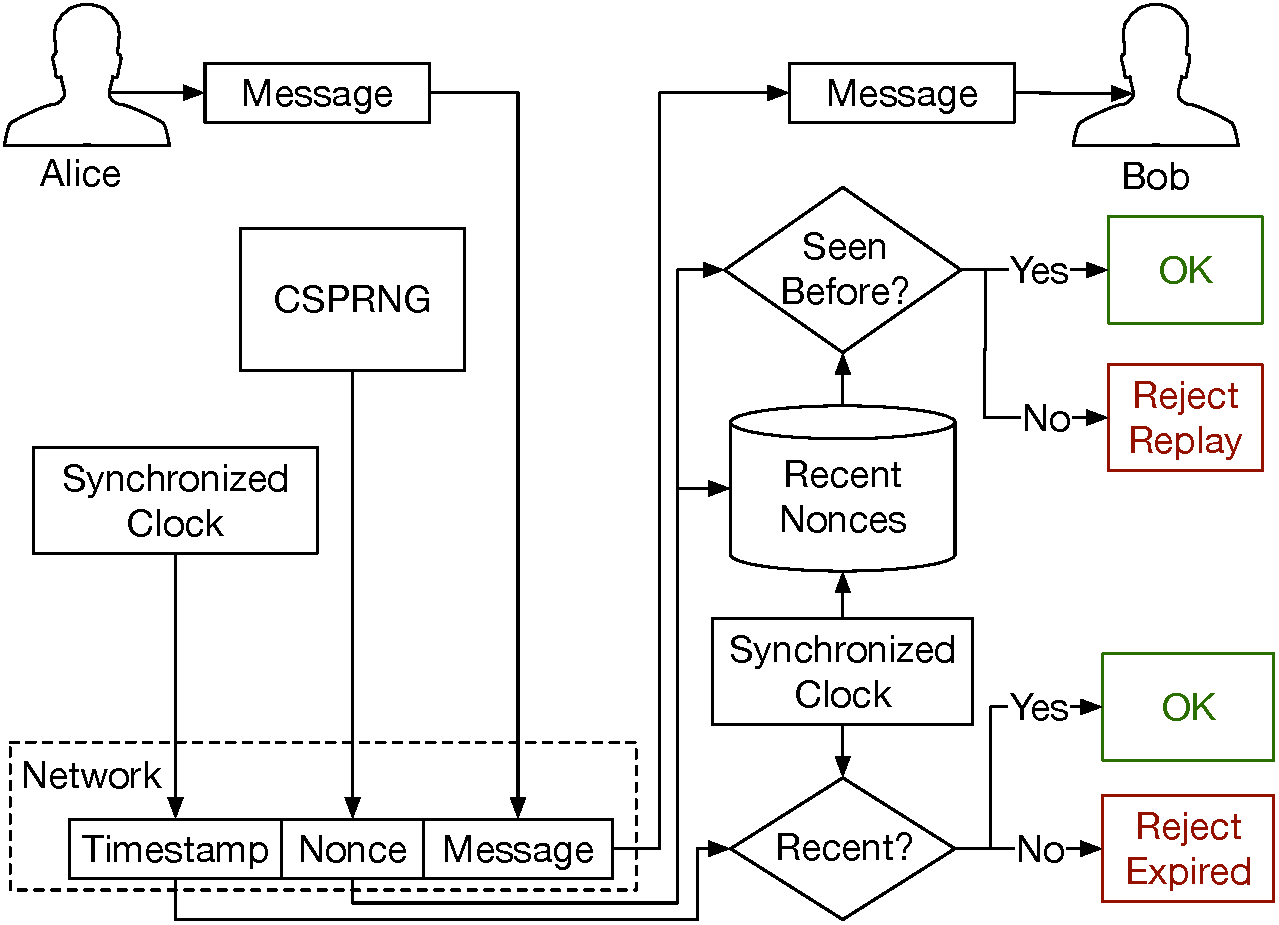
\includegraphics[width=87mm]{figures/timestamped_nonces.pdf}
  \caption{
    Freshness guarantees can be obtained by adding timestamped nonces on top
    of a system that already offers integrity guarantees. The sender and the
    receiver use synchronized clocks to timestamp each message and discard
    unreasonably old messages. The receiver must check the nonce in each new
    message against a database of the nonces in all the unexpired messages that
    it has seen.
  }
  \label{fig:timestamped_nonces}
\end{figure}

Alternatively, nonces can be used in challenge-response protocols, in a manner
that removes the storage overhead concerns. The challenger generates a nonce
and embeds it in the challenge message. The response to the challenge includes
an acknowledgement of the embedded nonce, so the challenger can distinguish
between a fresh response and a replay attack. The nonce is only stored by the
challenger, and is small in comparison to the rest of the state needed to
validate the response.
